% !TeX program = xelatex
\documentclass[a4paper,10pt]{article}

% ============================================================================
% កញ្ចប់បណ្ណាល័យ (Packages) – តាមលំនាំស្តង់ដារ អនុវិទ្យាល័យព្រះក្រសាំង (ls_plan.tex)
% បរិបទ៖ ថ្នាក់រៀនគ្មានស្លាយ LCD – បង្រៀនដោយប្រើក្ដារខៀន សៀវភៅគោល និងសន្លឹកកិច្ចការស-ខ្មៅ
% ============================================================================
\usepackage[a4paper, left=0.95cm, right=0.95cm, top=0.85cm, bottom=0.92cm, footskip=0.52cm]{geometry}
\usepackage{amsmath, amssymb}
\usepackage{unicode-math}
\usepackage{fontspec}
\usepackage{array, longtable, multirow, colortbl}
\usepackage[table]{xcolor}
\usepackage{enumitem}
\usepackage{pifont}
\usepackage{fancyhdr}
\usepackage{tikz}
\usetikzlibrary{calc, arrows.meta, positioning, babel}

\makeatletter
\let\@expl@@@mark@update@singlecol@structures@@\relax
\makeatother

\providecommand{\NGSFindFonts}{%
  \IfFileExists{C:/Windows/Fonts/cambria.ttc}{%
    \def\NGSSysPath{C:/Windows/Fonts/}%
    \def\NGSUserPath{C:/Users/KIT/AppData/Local/Microsoft/Windows/Fonts/}%
  }{%
    \IfFileExists{./fonts/KhmerOSsiemreap.ttf}{\def\NGSSysPath{./fonts/}\def\NGSUserPath{./fonts/}}{%
    \IfFileExists{../fonts/KhmerOSsiemreap.ttf}{\def\NGSSysPath{../fonts/}\def\NGSUserPath{../fonts/}}{%
    \IfFileExists{../../fonts/KhmerOSsiemreap.ttf}{\def\NGSSysPath{../../fonts/}\def\NGSUserPath{../../fonts/}}{%
    \IfFileExists{../../../fonts/KhmerOSsiemreap.ttf}{\def\NGSSysPath{../../../fonts/}\def\NGSUserPath{../../../fonts/}}{%
    \IfFileExists{../../../../fonts/KhmerOSsiemreap.ttf}{\def\NGSSysPath{../../../../fonts/}\def\NGSUserPath{../../../../fonts/}}{%
    \IfFileExists{../../../../../fonts/KhmerOSsiemreap.ttf}{\def\NGSSysPath{../../../../../fonts/}\def\NGSUserPath{../../../../../fonts/}}{%
    \IfFileExists{../../../../../../fonts/KhmerOSsiemreap.ttf}{\def\NGSSysPath{../../../../../../fonts/}\def\NGSUserPath{../../../../../../fonts/}}{%
      \def\NGSSysPath{../../../../../../../fonts/}\def\NGSUserPath{../../../../../../../fonts/}%
    }}}}}}}%
  }%
}
\NGSFindFonts

\setmathfont[Path={\NGSSysPath}, FontIndex=1, Scale=1.02]{cambria.ttc}
\defaultfontfeatures{Ligatures=TeX}

\setmainfont[
  Path={\NGSUserPath},
  Extension=.ttf,
  Script=Khmer,
  BoldFont={KhmerOSsiemreap},
  BoldFeatures={FakeBold=1.8},
  ItalicFont={KhmerOSsiemreap},
  ItalicFeatures={FakeSlant=0.25},
  BoldItalicFont={KhmerOSsiemreap},
  BoldItalicFeatures={FakeBold=1.8, FakeSlant=0.25}
]{KhmerOSsiemreap}

\newfontfamily\muol[Path={\NGSUserPath}, Extension=.ttf, Script=Khmer]{KhmerOSmuollight}
\newfontfamily\TimesEn[Path={\NGSSysPath}, Extension=.ttf, BoldFont={timesbd}, ItalicFont={timesi}, BoldItalicFont={timesbi}]{times}
\newfontfamily\NagaBold[Path={\NGSUserPath}, Extension=.ttf]{AKbalthom Naga Bold}
\newfontfamily\CalibriFont[Path={\NGSSysPath}, Extension=.ttf]{calibri}
\newfontfamily\Tacteing[Path={\NGSUserPath}]{TACTENG.TTF}
\newfontfamily\CourierBullet[Path={\NGSSysPath}, Extension=.ttf]{cour}
\newcommand{\wcirc}{{\CourierBullet\fontsize{9.5pt}{11pt}\selectfont o}}

\XeTeXlinebreaklocale "km"
\XeTeXlinebreakskip = 0pt plus 1pt minus 0.1pt

\definecolor{stepgray}{HTML}{D9D9D9}
\definecolor{headgray}{HTML}{F2F2F2}
\definecolor{boxgray}{HTML}{D9D9D9}
\definecolor{darkred}{HTML}{C00000}
\definecolor{red5e}{HTML}{FF0000}

\pagestyle{fancy}
\fancyhf{}
\renewcommand{\headrulewidth}{0pt}
\fancyfoot[R]{\CalibriFont\fontsize{11pt}{13pt}\selectfont\thepage}

\setlength{\parindent}{0pt}
\setlength{\parskip}{0pt}
\setlength{\tabcolsep}{3.8pt}

\newcolumntype{L}[1]{>{\raggedright\arraybackslash}p{#1}}

\newcommand{\en}[1]{{\TimesEn #1}}
\newcommand{\enbf}[1]{{\TimesEn\textbf{#1}}}
\newcommand{\unit}[1]{\,\text{\en{#1}}}
\newcommand{\fiveE}[1]{{\NagaBold\fontsize{9.5pt}{13pt}\selectfont\textcolor{red5e}{#1}}}
\newcommand{\timenote}[1]{\textcolor{darkred}{\textit{#1}}}
\newcommand{\graybox}[1]{\colorbox{boxgray}{\strut\hspace{2pt}#1\hspace{2pt}}}
\newcommand{\ditem}{\tikz[baseline=-0.5ex]\fill (0,0.42ex) -- (0.42ex,0) -- (0,-0.42ex) -- (-0.42ex,0) -- cycle;\hspace{0.3em}}
\newcommand{\cnum}[1]{{\fontsize{10.5pt}{12pt}\selectfont\ding{\numexpr171+#1\relax}}\hspace{0.2em}}
\newcommand{\cfig}[1]{\par\vspace{4pt}{\centering #1\par}\vspace{4pt}}
\newcommand{\stepheader}[1]{\multicolumn{3}{|c|}{\cellcolor{stepgray}\muol #1} \\* \noalign{\hrule height 0.4pt}}
\newcommand{\khmflourish}{{\Tacteing\fontsize{36pt}{14pt}\selectfont\raisebox{-5pt}{3}}}

% ============================================================================
% ម៉ាក្រូរូបភាពគរុកោសល្យស-ខ្មៅ (Proportional B&W TikZ Diagrams)
% ============================================================================

% ១. E1 Engage: រងបន្លែរួមទទឹង 3m និងដំណើរបញ្ច្រាសពីពន្លាតទៅផលគុណកត្តា (ទំ.៦៨-៦៩)
\newcommand{\figEngageALGSeven}{%
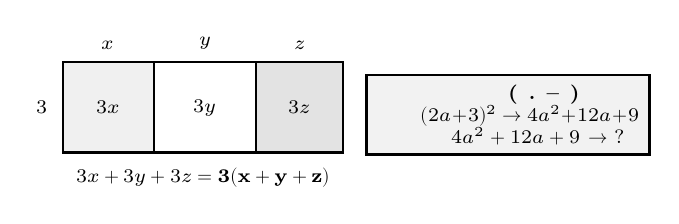
\begin{tikzpicture}[every node/.style={font=\scriptsize, text=black}]
  \begin{scope}
    \draw[line width=0.9pt, fill=gray!12] (0,0) rectangle (1.15,1.15);
    \draw[line width=0.9pt, fill=white] (1.15,0) rectangle (2.45,1.15);
    \draw[line width=0.9pt, fill=gray!22] (2.45,0) rectangle (3.55,1.15);
    \node at (0.57,0.57) {$3x$};
    \node at (1.80,0.57) {$3y$};
    \node at (3.00,0.57) {$3z$};
    \node[left=2pt] at (0,0.57) {$3$};
    \node[above=1pt] at (0.57,1.15) {$x$};
    \node[above=1pt] at (1.80,1.15) {$y$};
    \node[above=1pt] at (3.00,1.15) {$z$};
    \node[below=2pt, font=\scriptsize] at (1.78,0) {$3x+3y+3z = \mathbf{3(x+y+z)}$};
  \end{scope}
  \node[draw=black, line width=0.9pt, fill=gray!10, text width=3.35cm, align=center, inner sep=3.5pt] at (5.65,0.48) {
    \textbf{ដំណើរបញ្ច្រាស (ទំ.៦៨--៦៩)៖}\\
    ពន្លាត៖ $(2a+3)^2 \to 4a^2+12a+9$\\
    ដាក់កត្តា៖ $4a^2+12a+9 \to \mathbf{?}$
  };
\end{tikzpicture}}

% ២. E4 Elaborate: មែកធាងសម្រេចចិត្តដាក់ជាផលគុណកត្តា (GCF-First Decision Tree)
\newcommand{\figTreeALGSeven}{%
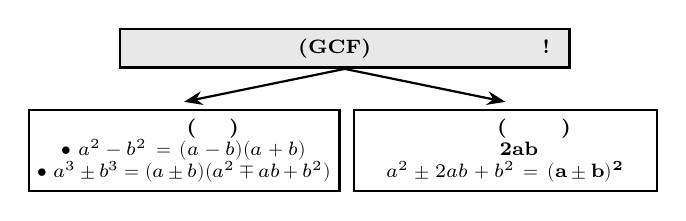
\begin{tikzpicture}[every node/.style={font=\scriptsize, text=black}, >=Stealth]
  \node[draw=black, line width=0.9pt, fill=gray!18, inner sep=3.5pt, align=center] (top) at (0,1.30) {
    \textbf{ជំហានទី១៖ ពិនិត្យចាប់កត្តារួម (\en{GCF}) ឬកញ្ចប់វង់ក្រចករួមជាមុនជានិច្ច!}
  };
  \node[draw=black, line width=0.8pt, fill=white, text width=3.72cm, inner sep=3.2pt, align=center] (two) at (-2.04,0) {
    \textbf{បើសល់ ២ តួ (ទ្វេធា)៖}\\
    $\bullet$ $a^2-b^2 = (a-b)(a+b)$\\
    $\bullet$ $a^3\pm b^3 = (a\pm b)(a^2\mp ab+b^2)$
  };
  \node[draw=black, line width=0.8pt, fill=white, text width=3.62cm, inner sep=3.2pt, align=center] (three) at (2.04,0) {
    \textbf{បើសល់ ៣ តួ (ត្រីធាការេ)៖}\\
    ផ្ទៀងតួកណ្ដាល $\mathbf{2ab}$ រួចដាក់៖\\
    $a^2\pm 2ab+b^2 = \mathbf{(a\pm b)^2}$
  };
  \draw[->, line width=0.8pt] (top.south) -- (-2.04,0.62);
  \draw[->, line width=0.8pt] (top.south) -- (2.04,0.62);
\end{tikzpicture}}

\begin{document}
\fontsize{10pt}{15.2pt}\selectfont

% -------------------- ក្បាលកិច្ចតែងការ (Header) --------------------
\begin{center}
  {\muol\fontsize{11pt}{16pt}\selectfont ព្រះរាជាណាចក្រកម្ពុជា}\\[2pt]
  {\muol\fontsize{10pt}{15pt}\selectfont ជាតិ សាសនា ព្រះមហាក្សត្រ}\\[1pt]
  \khmflourish
\end{center}

\vspace{-28pt}
{\muol\fontsize{9.5pt}{12.5pt}\selectfont
មន្ទីរអប់រំ យុវជន និងកីឡា ខេត្តកំពង់ធំ\\
ការិយាល័យអប់រំ យុវជន និងកីឡា ស្រុកកំពង់ស្វាយ\\
អនុវិទ្យាល័យព្រះក្រសាំង}

\vspace{1pt}
\begin{center}
  {\muol\fontsize{10pt}{14pt}\selectfont កិច្ចតែងការបង្រៀន}
\end{center}
\vspace{0pt}

% -------------------- ព័ត៌មានទូទៅ (Metadata) --------------------
{\renewcommand{\arraystretch}{0.95}
\hspace*{4.05cm}%
\begin{tabular}{@{}l l l@{}}
  - \hspace{0.35cm} មុខវិជ្ជា & : & គណិតវិទ្យា ថ្នាក់ទី៨ \\
  - \hspace{0.35cm} ចំណងជើងមេរៀន & : & មេរៀនទី៥ កន្សោមពីជគណិត \\
  - \hspace{0.35cm} ចំណងជើងរង & : & ៤.១ និង ៤.២ ការដាក់ជាផលគុណកត្តាដោយកត្តារួម និងសមភាពសំខាន់ៗ \\
  - \hspace{0.35cm} រយៈពេល & : & ១ ម៉ោងសិក្សា (៥០ នាទី) \\
  - \hspace{0.35cm} បង្រៀនដោយ & : & ហុក ប៊ុនថែន \\
  - \hspace{0.35cm} កាលបរិច្ឆេទ & : & ថ្ងៃសុក្រ ២កើត ខែមិគសិរ ព.ស.២៥៧០ (១១ ធ្នូ ២០២៦) \\
\end{tabular}
}

\vspace{1pt}

% -------------------- I. វត្ថុបំណង --------------------
\textbf{I.} {\muol វត្ថុបំណង}\\[1pt]
\hspace*{0.55cm}%
\begin{tabular}{@{}l l L{14.2cm}@{}}
  \wcirc \hspace{0.25cm} វិជ្ជាសម្បទា & : & សិស្សប្រាប់បានត្រឹមត្រូវនូវនិយមន័យនៃការដាក់កន្សោមជាផលគុណកត្តា វិធីចាប់កត្តារួម (ឯកធា ឬទ្វេធាក្នុងវង់ក្រចក) និងលក្ខខណ្ឌប្រើសមភាពសំខាន់ៗ $(a\pm b)^2$, $a^2-b^2$, $a^3\pm b^3$ (ទំ.៦៨--៧០) ។ \\
  \wcirc \hspace{0.25cm} បំណិនសម្បទា & : & សិស្សដាក់កន្សោមពីជគណិតជាផលគុណកត្តាបានត្រឹមត្រូវដោយចាប់កត្តារួមជាមុន និងជ្រើសរើសសមភាពសំខាន់ៗសមស្របតាមចំនួនតួ (២ តួ ឬ ៣ តួ) ។ \\
  \wcirc \hspace{0.25cm} ចរិយាសម្បទា & : & សិស្សមានទម្លាប់ពិនិត្យកត្តារួម និងផ្ទៀងផ្ទាត់តួកណ្ដាល $2ab$ ដោយហ្មត់ចត់មុននឹងសន្និដ្ឋានថាជាការេនៃទ្វេធា ព្រមទាំងសហការពិភាក្សាដៃគូយ៉ាងសកម្ម ។ \\
\end{tabular}

\vspace{1pt}

% -------------------- II. សម្ភារៈឧបទេស --------------------
\textbf{II.} {\muol សម្ភារៈឧបទេស}\\[1pt]
\hspace*{0.55cm}$\bullet$ \hspace{0.35cm} សៀវភៅសិក្សាគោលគណិតវិទ្យាថ្នាក់ទី៨ (ទំ.៦៨--៧០ និងទំ.៧៣--៧៤) ក្ដារខៀន ដីស បន្ទាត់ និងសន្លឹកកិច្ចការសិស្សស-ខ្មៅ (\en{Worksheet\_ALG57} ចំនួន ២ ទំព័រ \en{A4} ដោយគ្មានស្លាយ \en{LCD}) ។

\vspace{1pt}

% -------------------- III. វិធីសាស្រ្តបង្រៀន --------------------
\textbf{III.} {\muol វិធីសាស្រ្តបង្រៀន}\\[1pt]
\hspace*{0.55cm}$\bullet$ \hspace{0.35cm} គោលវិធីសិស្សមជ្ឈមណ្ឌលតាមគំរូ \en{5Es} រួមបញ្ចូល \textbf{ការចាប់បណ្ដុំវង់ក្រចកជាកញ្ចប់ និងមែកធាងសម្រេចចិត្តដាក់ជាផលគុណកត្តា} (\en{Compound-Bracket Chunking \& GCF-First Factoring Decision Tree}; \en{Theba et al., 2024; O'Connor \& Norton, 2016}) ។

\vspace{2pt}

% -------------------- IV. ដំណើរការបង្រៀន --------------------
\textbf{IV.} {\muol ដំណើរការបង្រៀន}\\[-6pt]

{\renewcommand{\arraystretch}{1.15}
\begin{longtable}{|L{5.50cm}|L{7.90cm}|L{4.80cm}|}
\hline
\multicolumn{1}{|c|}{\cellcolor{headgray}\muol សកម្មភាពគ្រូ} &
\multicolumn{1}{c|}{\cellcolor{headgray}\muol ខ្លឹមសារមេរៀន} &
\multicolumn{1}{c|}{\cellcolor{headgray}\muol សកម្មភាពសិស្ស} \\[2pt]
\hline
\endfirsthead

\hline
\multicolumn{1}{|c|}{\cellcolor{headgray}\muol សកម្មភាពគ្រូ} &
\multicolumn{1}{c|}{\cellcolor{headgray}\muol ខ្លឹមសារមេរៀន} &
\multicolumn{1}{c|}{\cellcolor{headgray}\muol សកម្មភាពសិស្ស} \\[2pt]
\hline
\endhead

\hline
\endfoot

% ==================== ជំហានទី១ (2min) ====================
\stepheader{ជំហានទី១ ៖ រដ្ឋបាលថ្នាក់ (២ នាទី)}
$\bullet$ ពិនិត្យអវត្តមាន សណ្ដាប់ធ្នាប់ អនាម័យ និងសៀវភៅគោល \par\vspace{1pt}
$\bullet$ ចែកសន្លឹកកិច្ចការស-ខ្មៅ \en{Worksheet\_ALG57} ដល់សិស្សគ្រប់គ្នា
&
$\bullet$ វត្តមានសិស្ស ឯកសណ្ឋាន និងសណ្ដាប់ធ្នាប់ថ្នាក់រៀន \par
$\bullet$ សន្លឹកកិច្ចការសិស្ស \en{Worksheet\_ALG57} (ទំព័រ ១--២) លើតុរៀងៗខ្លួន
&
$\circ$ ប្រធានថ្នាក់រាយការណ៍អវត្តមាន \par
$\circ$ សរសេរឈ្មោះលើសន្លឹកកិច្ចការ \\
\hline

% ==================== ជំហានទី២ (9min) ====================
\stepheader{ជំហានទី២ ៖ កែកិច្ចការផ្ទះ រំលឹកមេរៀនចាស់ និងភ្ជាប់បញ្ហាថ្មី (៩ នាទី)}
\ditem \textbf{កែកិច្ចការផ្ទះ ($\le 3\unit{min}$)៖} \par
$\bullet$ ហៅសិស្ស ១ រូបឡើងកែប្រតិបត្តិ ឃ (ទំ.៦៧) និងលំហាត់ ១០ង (ទំ.៧៣) លើក្ដារខៀន
&
\textbf{កំណែកិច្ចការផ្ទះ (សៀវភៅគោល ទំ.៦៧ និងទំ.៧៣)៖} \par
១) $(\sqrt{2}a + 3b)(2a^2 - 3\sqrt{2}ab + 9b^2) = (\sqrt{2}a)^3 + (3b)^3 = \mathbf{2\sqrt{2}a^3 + 27b^3}$ ។ \par
២) $(x-1)^3 - (x+2)^3 = (x^3-3x^2+3x-1) - (x^3+6x^2+12x+8) = \mathbf{-9x^2 - 9x - 9}$ ។
&
$\circ$ ផ្ទៀងផ្ទាត់ការប្ដូរសញ្ញាក្រោយសញ្ញាដក និងកែលម្អចម្លើយ \\[3pt]

\ditem \textbf{រំលឹកមេរៀនចាស់ ($3\unit{min}$)៖} \par
$\bullet$ សួររំលឹកសមភាពសំខាន់ៗទាំង ៥ ក្នុងប្រអប់សង្ខេបទំ.៦៨ និងលក្ខណៈបំបែក $k(a+b)$
&
\textbf{សំណួររំលឹកមូលដ្ឋានគ្រឹះ (ទំ.៦៨)៖} \par
១) លក្ខណៈបំបែក៖ $k(x + y + z) = kx + ky + kz$ ។ \par
២) សមភាពសំខាន់ៗ៖ $(a\pm b)^2 = a^2\pm 2ab+b^2$, $a^2-b^2 = (a-b)(a+b)$ និង $a^3\pm b^3 = (a\pm b)(a^2\mp ab+b^2)$ ។
&
$\circ$ ឆ្លើយរំលឹករូបមន្តសង្ខេបទាំង ៥ ដោយមើលពីអង្គស្ដាំទៅអង្គឆ្វេង \\[3pt]

\fiveE{E1 - Engage} \timenote{(3 នាទី)} \par\vspace{1pt}
$\bullet$ គូររងបន្លែ ៣ ជាប់គ្នា ($3x+3y+3z$) និងកន្សោម $(3x+2y)(x+1) - y(x+1)$ លើក្ដារខៀន រួចឱ្យសិស្សទស្សន៍ទាយវិធីដាក់ជាផលគុណកត្តាដោយមិនបាច់គុណពន្លាត
&
\textbf{ស្ថានភាពភ្ជាប់បញ្ហា៖ ដំណើរបញ្ច្រាសពីផលបូកទៅផលគុណកត្តា!} \par
រងបន្លែ ៣ ជាប់គ្នាមានក្រឡាផ្ទៃសរុប $3x + 3y + 3z$ និងរួមទទឹង $3\unit{m}$ ដូចគ្នា ។ ចុះបើជួបកន្សោម $(3x+2y)(x+1) - y(x+1)$ ឬត្រីធា $4a^2 + 12a + 9$ តើយើងអាចបំប្លែងទៅជាផលគុណកត្តាដឺក្រេទី១ ភ្លាមដោយរបៀបណា? \par
\hspace*{0.3em}– \textbf{សំណួរបេសកកម្ម៖} «តើ $(x+1)$ អាចចាប់ជាកត្តារួមទាំងកញ្ចប់បានឬទេ? ហើយតើត្រីធាគ្រប់រូបសុទ្ធតែស្មើ $(a\pm b)^2$ មែនឬទេ?»
&
$\circ$ សង្កេតកត្តារួម $3$ និងកញ្ចប់ $(x+1)$ \par
$\circ$ គូសធីកការទស្សន៍ទាយមុនរៀនក្នុងផ្នែកទី១ នៃសន្លឹកកិច្ចការ \\[3pt]

& \cfig{\figEngageALGSeven} & \\
\hline

% ==================== ជំហានទី៣ (17min) ====================
\stepheader{ជំហានទី៣ ៖ មេរៀនថ្មី — ការដាក់ជាផលគុណកត្តាដោយកត្តារួម និងសមភាពសំខាន់ៗ (១៧ នាទី)}
\fiveE{E2 - Explore} \timenote{(11 នាទី)} \par\vspace{1pt}
\ditem \textbf{សកម្មភាពទី១៖ រុករកកត្តារួមឯកធា និងកញ្ចប់វង់ក្រចក ($5.5\unit{min}$)៖} \par
$\bullet$ ឱ្យសិស្សធ្វើការជាដៃគូលើ \textbf{ផ្នែកទី២ (ក)} នៃ \en{Worksheet\_ALG57} ដើម្បីចាប់កត្តារួមក្នុងឧទាហរណ៍ទី១--២ និងលំហាត់គំរូ (ទំ.៦៨--៦៩)
&
\textbf{ការរុករកទី១ (៤.១ កត្តារួម ទំ.៦៨--៦៩)៖} \par
$\bullet$ ឧទាហរណ៍១៖ $3x + 3y + 3z = \mathbf{3(x + y + z)}$ (ហៅថាផលគុណកត្តា) ។ \par
$\bullet$ ឧទាហរណ៍២៖ $x\underline{(2b-3)} + y\underline{(2b-3)} = \mathbf{(2b-3)(x + y)}$ ។ \par
$\bullet$ លំហាត់គំរូ (ទំ.៦៩)៖ $(3x+2y)\underline{(x+1)} - y\underline{(x+1)} = (x+1)(3x+2y-y) = \mathbf{(x+1)(3x+y)}$ ។
&
$\circ$ គូសបន្ទាត់ក្រោមកញ្ចប់ $(2b-3)$ និង $(x+1)$ រួចដាក់ជាកត្តារួម \par
$\circ$ បង្រួមតួដូចគ្នា $2y - y = y$ ក្នុងវង់ក្រចកទី២ \\[3pt]

\ditem \textbf{សកម្មភាពទី២៖ រុករកការដាក់កត្តាតាមសមភាពសំខាន់ៗ ($5.5\unit{min}$)៖} \par
$\bullet$ ឱ្យដៃគូបន្តបំពេញ \textbf{ផ្នែកទី២ (ខ)}៖ ផ្ទៀងផ្ទាត់តួកណ្ដាល $2ab$ ចំពោះត្រីធា (ទំ.៦៩) និងបំបែកផលបូក-ដកពីរគូប (ទំ.៧០)
&
\textbf{ការរុករកទី២ (៤.២ ប្រើសមភាពសំខាន់ៗ ទំ.៦៩--៧០)៖} \par
$\bullet$ $4a^2 + 12a + 9 = (2a)^2 + 2(2a)(3) + 3^2 = (2a+3)^2 = \mathbf{(2a+3)(2a+3)}$ ។ \par
$\bullet$ $\frac{x^2}{4} - 4x + 16 = \left(\frac{x}{2}\right)^2 - 2\left(\frac{x}{2}\right)(4) + 4^2 = \mathbf{\left(\frac{x}{2}-4\right)\left(\frac{x}{2}-4\right)}$ ។ \par
$\bullet$ គូប (ទំ.៧០)៖ $8x^3 + y^3 = (2x)^3 + y^3 = \mathbf{(2x+y)(4x^2-2xy+y^2)}$ និង $27y^3 - 64 = (3y)^3 - 4^3 = \mathbf{(3y-4)(9y^2+12y+16)}$ ។
&
$\circ$ ផ្ទៀងផ្ទាត់ឃើញ $x^2 + 6x + 16$ មិនមែនជាការេទ្វេធាទេ (ព្រោះ $2(x)(4) = 8x \ne 6x$) \par
$\circ$ ប្រៀបធៀបសញ្ញាក្នុងកត្តានៃ $8x^3+y^3$ និង $27y^3-64$ \\[3pt]

\fiveE{E3 - Explain} \timenote{(6 នាទី)} \par\vspace{1pt}
$\bullet$ ហៅតំណាងដៃគូឡើងសង្ខេបនិយមន័យ និងជំហានចាប់កត្តារួមលើក្ដារខៀន
&
\textbf{សង្ខេបខ្លឹមសារគោល៖ វិធានដាក់ជាផលគុណកត្តា (ទំ.៦៨--៧០)} \par
$\bullet$ \cnum{1} \textbf{ចាប់កត្តារួមជាមុនជានិច្ច៖} $ka + kb = k(a + b)$ ដែល $k$ អាចជាចំនួន ឯកធា ឬកញ្ចប់ទ្វេធា ។ \par
$\bullet$ \cnum{2} \textbf{ករណី ២ តួ (ផលដកពីរការេ)៖} $a^2 - b^2 = (a - b)(a + b)$ \textit{(ខណៈ $a^2+b^2$ មិនអាចដាក់ជាកត្តាដឺក្រេទី១ ទេ!)} ។
&
$\circ$ ឡើងសរសេរវិធានចាប់កត្តារួម និងផលដកពីរការេលើក្ដារខៀន \\[3pt]

$\bullet$ សង្ខេបវិធានដាក់កត្តាសម្រាប់ផលបូក-ដកពីរគូប និងត្រីធាការេទ្វេធា
&
$\bullet$ \cnum{3} \textbf{ករណី ២ តួ (ផលបូក-ដកពីរគូប)៖} $a^3 \pm b^3 = (a \pm b)(a^2 \mp ab + b^2)$ ។ \par
$\bullet$ \cnum{4} \textbf{ករណី ៣ តួ (ត្រីធាការេទ្វេធា)៖} ពិនិត្យតួចុងទាំងពីរជាការេ $a^2, b^2$ និងផ្ទៀងតួកណ្ដាលស្មើ $\pm 2ab$ រួចដាក់ $a^2 \pm 2ab + b^2 = (a \pm b)^2$ ។
&
$\circ$ កត់ត្រាវិធាន \cnum{1}--\cnum{4} ចូលក្នុងប្រអប់ផ្នែកទី៣ នៃសន្លឹកកិច្ចការ \\
\hline

% ==================== ជំហានទី៤ (20min) ====================
\stepheader{ជំហានទី៤ ៖ ពង្រីកចំណេះដឹង និងវាយតម្លៃលទ្ធផលសិក្សា (២០ នាទី)}
\fiveE{E4 - Elaborate} \timenote{(10 នាទី)} \par\vspace{1pt}
\ditem \textbf{លំហាត់គំរូទី ១ និងទី ២ — ការេទ្វេធា និងរ៉ាឌីកាល់ (ទំ.៦៩--៧០, $5\unit{min}$)៖} \par
$\bullet$ ដឹកនាំសិស្សដោះស្រាយលំហាត់គំរូទី១ និងទី២ ក្នុង \textbf{ផ្នែកទី៤ (១)} នៃសន្លឹកកិច្ចការ
&
\textbf{លំហាត់គំរូទី ១ និងទី ២ (សៀវភៅគោល ទំ.៦៩--៧០)៖} \par
$\bullet$ គំរូ១៖ ក) $x^2 + 10x + 25 = \mathbf{(x+5)(x+5)}$ \;;\; ខ) $x^2 - 20x + 100 = \mathbf{(x-10)(x-10)}$ ។ \par
$\bullet$ គំរូ២ ក៖ $4x^2 - 16xy + 16y^2 = (2x - 4y)^2 = [2(x-2y)]^2 = \mathbf{4(x - 2y)^2}$ ។ \par
$\bullet$ គំរូ២ ខ៖ $2m^2 + \sqrt{2}mn + \frac{n^2}{4} = (\sqrt{2}m)^2 + 2(\sqrt{2}m)\left(\frac{n}{2}\right) + \left(\frac{n}{2}\right)^2 = \mathbf{\left(\sqrt{2}m + \frac{n}{2}\right)^2}$ ។
&
$\circ$ កត់សម្គាល់ថាបើចាប់កត្តារួម $4$ ចេញពី $4x^2-16xy+16y^2$ ជាមុន នោះបាន $4(x^2-4xy+4y^2) = 4(x-2y)^2$ កាន់តែងាយ! \\[3pt]

\ditem \textbf{លំហាត់គំរូគូប និងការគួបផ្សំកត្តារួមជាមួយសមភាព (ទំ.៧០, ៧៤, $5\unit{min}$)៖} \par
$\bullet$ ដឹកនាំសិស្សដោះស្រាយលំហាត់គំរូគូប (ទំ.៧០) និងករណីចាប់កត្តារួមមុនប្រើសមភាព (ទំ.៧៤)
&
\textbf{លំហាត់គំរូគូប និងករណីពីរដំណាក់កាល (ទំ.៧០ និងទំ.៧៤)៖} \par
$\bullet$ គំរូគូប (ទំ.៧០)៖ ក) $x^3 - 27 = \mathbf{(x-3)(x^2+3x+9)}$ \;;\; ខ) $8a^3 + 1 = \mathbf{(2a+1)(4a^2-2a+1)}$ ។ \par
$\bullet$ ចាប់កត្តារួមរួចបំបែកត (១៣ច, ១៤ង ទំ.៧៤)៖ $5x^3 - 80x = 5x(x^2 - 16) = \mathbf{5x(x-4)(x+4)}$ និង $a^2c - 2acx + cx^2 = c(a^2 - 2ax + x^2) = \mathbf{c(a - x)^2}$ ។ \par
$\bullet$ \textbf{ឆ្លុះបញ្ចាំង៖} កត្តាត្រីធា $x^2+3x+9$ នៃ $x^3-27$ មិនអាចបំបែកជា $(x+3)^2$ ទេ ព្រោះតួកណ្ដាលគឺ $+3x \ne +6x$!
&
$\circ$ អនុវត្តមែកធាងសម្រេចចិត្ត៖ ចាប់កត្តារួម $5x$ និង $c$ ចេញសិន ទើបឃើញសមភាពសំខាន់ៗភ្លាម \\[3pt]

& \cfig{\figTreeALGSeven} & \\[3pt]

\fiveE{E5 - Evaluate} \timenote{(10 នាទី)} \par\vspace{1pt}
\ditem \textbf{អនុវត្ត «ប្រតិបត្តិ» ទំ.៧០ និងលំហាត់សំយោគ ($6.5\unit{min}$)៖} \par
$\bullet$ ឱ្យសិស្សធ្វើលំហាត់ \textbf{ប្រតិបត្តិ} (ទំ.៧០) ដោយខ្លួនឯងក្នុងផ្នែកទី៥ (១) នៃសន្លឹកកិច្ចការ
&
\textbf{ចម្លើយលំហាត់ «ប្រតិបត្តិ» ទំ.៧០ និងសំយោគ (ទំ.៧៣--៧៤)៖} \par
១) \textbf{ប្រតិបត្តិការេទ្វេធា (ទំ.៧០)៖} ក) $x^2 - 8x + 16 = \mathbf{(x-4)(x-4)}$ \;;\; ខ) $y^2 + 10y + 25 = \mathbf{(y+5)(y+5)}$ \;;\; គ) $n^2 - 12n + 36 = \mathbf{(n-6)(n-6)}$ \;;\; ឃ) $a^2 + 16a + 64 = \mathbf{(a+8)(a+8)}$ \;;\; ង) $4x^2 + 12xy + 9y^2 = \mathbf{(2x+3y)^2}$ ។
&
$\circ$ ផ្ទៀងតួកណ្ដាល $2ab$ រួចសរសេរជាផលគុណកត្តាដឺក្រេទី១ \\[3pt]

$\bullet$ ឱ្យសិស្សបន្តធ្វើលំហាត់កត្តារួម និងសមភាពពីរតួ រួចប្ដូរសន្លឹកកិច្ចការផ្ទៀងជាដៃគូ
&
២) \textbf{កត្តារួម និងទ្វេធាការេ-គូប៖} \par
\hspace*{0.3em}– ក) $x(4x - 8y) + y(x - 2y) = 4x(x - 2y) + y(x - 2y) = \mathbf{(x - 2y)(4x + y)}$ \;;\; ខ) $9x^2 - 4 = \mathbf{(3x-2)(3x+2)}$ \par
\hspace*{0.3em}– គ) $(x + 1)^2 - 4 = \mathbf{(x - 1)(x + 3)}$ \;;\; ឃ) $27x^3 + 1 = \mathbf{(3x + 1)(9x^2 - 3x + 1)}$ \;;\; ង) $1 - 8b^3 = \mathbf{(1-2b)(1+2b+4b^2)}$ ។
&
$\circ$ ប្ដូរសន្លឹកកិច្ចការផ្ទៀងផ្ទាត់ការចាប់ $4$ ចេញពី $(4x-8y)$ (\en{Pause-Review}) \\[3pt]

\ditem \textbf{បិទបេសកកម្ម E1 និងតេស្តរហ័ស \en{Exit Check} ($3.5\unit{min}$)៖} \par
$\bullet$ សួរបិទបេសកកម្ម E1 និងឱ្យសិស្សគូសរង្វង់ជម្រើស \en{A--D}
&
$\bullet$ \textbf{បិទបេសកកម្ម E1៖} $(3x+2y)(x+1) - y(x+1) = \mathbf{(x+1)(3x+y)}$ ហើយមិនមែនគ្រប់ត្រីធាសុទ្ធតែស្មើ $(a\pm b)^2$ ទេ (ត្រូវផ្ទៀង $2ab$) ។ \par
$\bullet$ \textbf{Exit Check៖} តើការដាក់កន្សោម $3x^2 - 12$ ជាផលគុណកត្តាដឺក្រេទី១ ពេញលេញត្រូវនឹងជម្រើសណា? \par
\en{A.} $3(x^2 - 4)$ \quad \en{B.} $3(x - 2)^2$ \quad \graybox{\enbf{C.} $3(x - 2)(x + 2)$ \ding{51}} \quad \en{D.} $(3x - 6)(x - 2)$
&
$\circ$ ចាប់កត្តារួម $3$ បាន $3(x^2-4)$ រួចបំបែកបន្តបានជម្រើស \textbf{C} \\
\hline

% ==================== ជំហានទី៥ (<=2min) ====================
\stepheader{ជំហានទី៥ ៖ កិច្ចការផ្ទះ និងបណ្ដាំផ្ញើ ($\le$ ២ នាទី)}
$\bullet$ កត់ត្រាកិច្ចការផ្ទះលើក្ដារខៀន (មានបោះពុម្ពស្រាប់នៅផ្នែកទី៦ នៃសន្លឹកកិច្ចការទំព័រទី២) \par
$\bullet$ រំលឹកឱ្យចាប់កត្តារួមក្នុងវង់ក្រចកជាមុនចំពោះលំហាត់ ១១ខ និង ១៣ច
&
\textbf{កិច្ចការផ្ទះ (សៀវភៅសិក្សាគោល ទំ.៧៣--៧៤)៖} \par
១. \textbf{លំហាត់ទី១១ (ក, ខ) ទំ.៧៣៖} ក) $9(2x+1) - 16(2x+1)^2$ \;;\; ខ) $(3a^2 - 12a) - 5(a - 4)$ ។ \par
២. \textbf{លំហាត់ទី១៣ (ក, ខ, ច, ឋ) ទំ.៧៤៖} ក) $a^2 - 25$ \;;\; ខ) $4b^2 - 1$ \;;\; ច) $5x^3 - 80x$ \;;\; ឋ) $9a^2 - (a+2)^2$ ។ \par
៣. \textbf{លំហាត់ទី១៤ គ (ទំ.៧៤)៖} ដាក់ជាផលគុណកត្តា $12abx - 6ax^2 + 3a^2x$ ។
&
$\circ$ កត់ត្រាកិច្ចការផ្ទះ និងទុកដាក់សន្លឹកកិច្ចការក្នុងសឺមីគណិតវិទ្យា \\[3pt]

$\bullet$ ណែនាំឱ្យអានចំណុច ៤.២ (ត) ជាមុនសម្រាប់ម៉ោងបញ្ចប់មេរៀនទី៥
&
$\bullet$ \textbf{អានជាមុន៖} ចំណុច \textbf{៤.២ (ត) របៀបផ្សេងៗក្នុងការដាក់កន្សោមជាផលគុណកត្តា} (បំពេញការេ បំបែកតួកណ្ដាល និងផ្ដុំតួ ទំព័រ ៧១--៧២) ។
&
$\circ$ ទទួលបណ្ដាំផ្ញើ និងជម្រាបលាគ្រូ \\

\end{longtable}
}

\vspace{6pt}

% -------------------- ហត្ថលេខា (Signature Block) --------------------
\begin{flushright}
\begin{minipage}{9.6cm}
\centering
ថ្ងៃសុក្រ ២កើត ខែមិគសិរ ឆ្នាំមមី អដ្ឋស័ក ពុទ្ធសករាជ ២៥៧០\\[2pt]
ព្រះក្រសាំង, ថ្ងៃទី១១ ខែធ្នូ ឆ្នាំ២០២៦\\[4pt]
{\muol គ្រូបង្រៀន}\\[32pt]
\hfill{\muol ហុក ប៊ុនថែន}\hspace*{1.4cm}
\end{minipage}
\end{flushright}

\end{document}
